\chapter{Konkurrenzanalyse}

In dieser Analyse wollen wir zunächst schauen welche Projektmanagement Software Produkte genug Marktanteile haben um für uns relevant zu sein. Wir ergründen dann wie wir unser Feature umsetzen wollen um uns danach anzuschauen wie die Konkurrenten in Ihren Produkten das Daily oder Weekly Meeting umgesetzt haben beziehungsweise in welcher Form die Arbeit in Projekten in den bestehenden Produkten dargestellt wird. Wir müssen uns dann noch mit der Frage beschäftigen in wie weit die Konkurrenzprodukte Vor- und Nachteile für unseren Kontext von Universitätsprojekten haben. Die für uns interessante Aspekte der Konkurrenz müssen wir dann evaluieren und entscheiden ob wir etwas vergleichbares auch in unser Produkt integrieren wollen.

\section{Aktueller Markt}

Der Markt für Projektmanagement Software in Deutschland besteht zu Dreivierteln aus 6 Produkten. \\
Dabei hat Jira von Atlassian den größten Martkanteil, der bei fast 50\% liegt. An zweiter Stelle liegt Microsoft Project mit etwa 12\% mit einigem Abstand folgt Kanban mit einem Martkanteil von etwa 7\%. Mit einem jeweiligen Marktanteil von 2-3\% folgen dann noch HPE ALM, Trello und Smartsheet. \\
In unserer Analyse werden wir uns mit den Top 3 beschäftigen also Jira, Microsoft Project und Kanban. 

\begin{figure}[H]
	\centering
	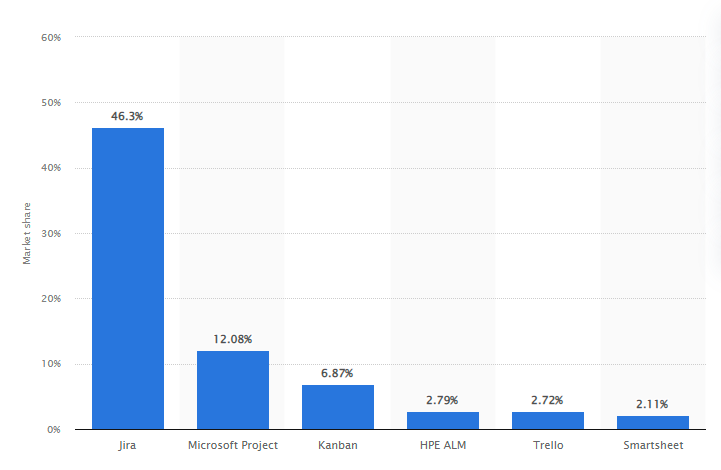
\includegraphics[width=0.95\textwidth]{marketshare.png}
    \caption{Marktanteil von Projektmanagement Software, Stand Januar 2020\cite{statista2020}}
	\label{fig:marketshare}
\end{figure}

\section{Das Weekly Standup}

Das wöchentliche beziehungsweise zweiwöchige Meeting dient dazu alle in der Projektgruppe auf dem laufenden zu halten, d.h. jedes Mitglied im Team dokumentiert für die anderen was gemacht wurde und erfährt im Gegenzug was die anderen gemacht haben.\\
Für den oder die Dozenten ist es ebenfalls wichtig zu sehen wie die Gruppe mit dem Projekt vorankommt und ob es Probleme gibt. Um den Fortschritt zu dokumentieren muss das Meeting in Schriftform stattfinden, denn wenn zum Beispiel ein Video von dem Meeting aufgezeichnet werden würde, dann wäre es ein erheblicher Aufwand für den Dozenten nachzuvollziehen was besprochen wurde. Es gibt zwar schon Technologien bei denen die gesagten Worte automatisch in Text umgewandelt werden allerdings sind diese nicht unbedingt verlässlich und darüber hinaus hat man am Ende nicht unbedingt ein strukturiertes Dokument um es auszuwerten.\\
Da es sich um Studenten und keine Mitarbeiter eines Unternehmens handelt ist auch nicht unbedingt davon auszugehen, dass alle Mitglieder in einer Gruppe zu einem festen Zeitpunkt an einem Meeting teilnehmen können oder während das Projekt läuft mit strikten Deadlines oder Sprints arbeiten werden oder können. Daher bietet es sich an das Meeting auch asynchron abzuhalten, dass heißt jeder Teilnehmer trägt unabhängig ein was seit dem letzten Meeting gemacht wurde, wo Probleme auftreten und was als nächstes gemacht wird beziehungsweise geplant ist. 

\section{Umsetzung des Daily/Weekly bei der Konkurrenz}

Wie haben die Konkurrenten das Daily/Weekly Meeting umgesetzt was können wir daraus lernen.

\subsection{Jira}

Da Jira der Marktführer ist schauen wir uns als erstes Jira im allgemeinen und die Features, die für Dailies sind im speziellen an. Jira existiert seit 2002 und hat sich als Marktführer bei Software Unternehmen etabliert. Neben den Standardfunktionalitäten bietet Jira außerdem Erweiterungen im Atlassian Marketplace an. Dabei handelt es sich um Applikationen, die Jira erweitern. Diese können von Atlassian selbst sein oder von Drittanbietern.\\
Jira geht davon aus, dass Teams entweder in Scrum oder Kanban arbeiten und bietet für diese beiden agilen Arbeitsmethoden Boards an. Die Features darum bauen auf dieser Annahme auf daher wird die Arbeit auch in Form von Tickets organisiert. Wenn ein User sich nicht an die vorgegebenen agilen Workflows hält stehen manche Funktionen wie zum Beispiel das Burn-Down Chart nicht zur Verfügung weil dafür zum Beispiel Story Points benötigt werden. Bei Studenten ist aber nicht davon auszugehen, dass sie zum einen wissen wie Story Points vergeben werden und zum andren bei so kurzen Implementierungsphasen wie es bei Projekten in der Universität der Fall ist eine aussagekräftige Schätzung abgeben können. \\
Jedes Ticket repräsentiert ein Arbeitspaket, welches im Board durch die verschiedenen Stadien im Workflow geht. Die Tickets sind wie es die Workflows vorgeben hierarchisch organisiert, d.h. es gibt verschiedene Ticket Typen wie Epic, Story, Bug und andere Tasks.

\begin{figure}[H]
	\centering
	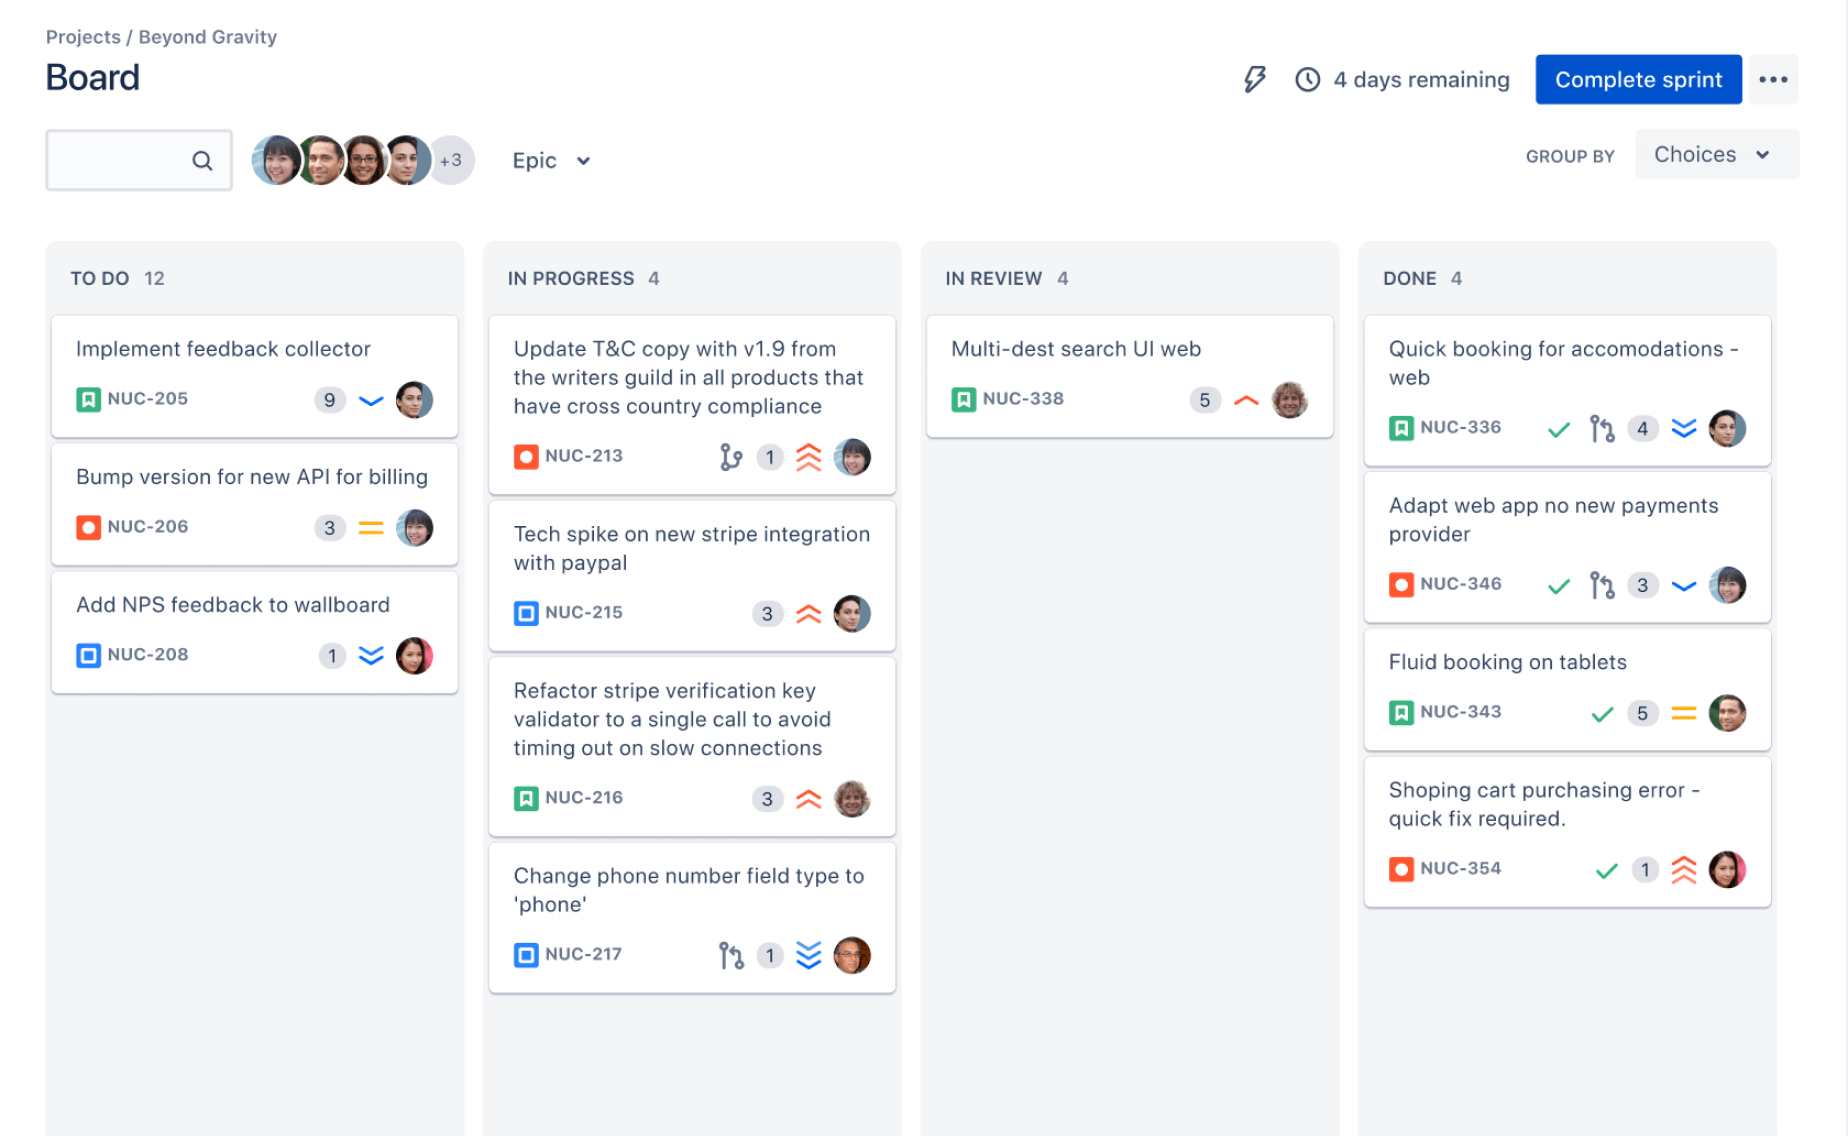
\includegraphics[width=0.95\textwidth]{jira-scrumboard.png}
    \caption{Scrum Board in Jira}
	\label{fig:scrumboardjira}
\end{figure}

Diese Ticket Typen haben eine bestimmte Hierarchie zum Beispiel kann eine Story zu einem Epic gehören und ein Bug Ticket kann ein Subtask einer Story sein. 

\begin{figure}[H]
	\centering
	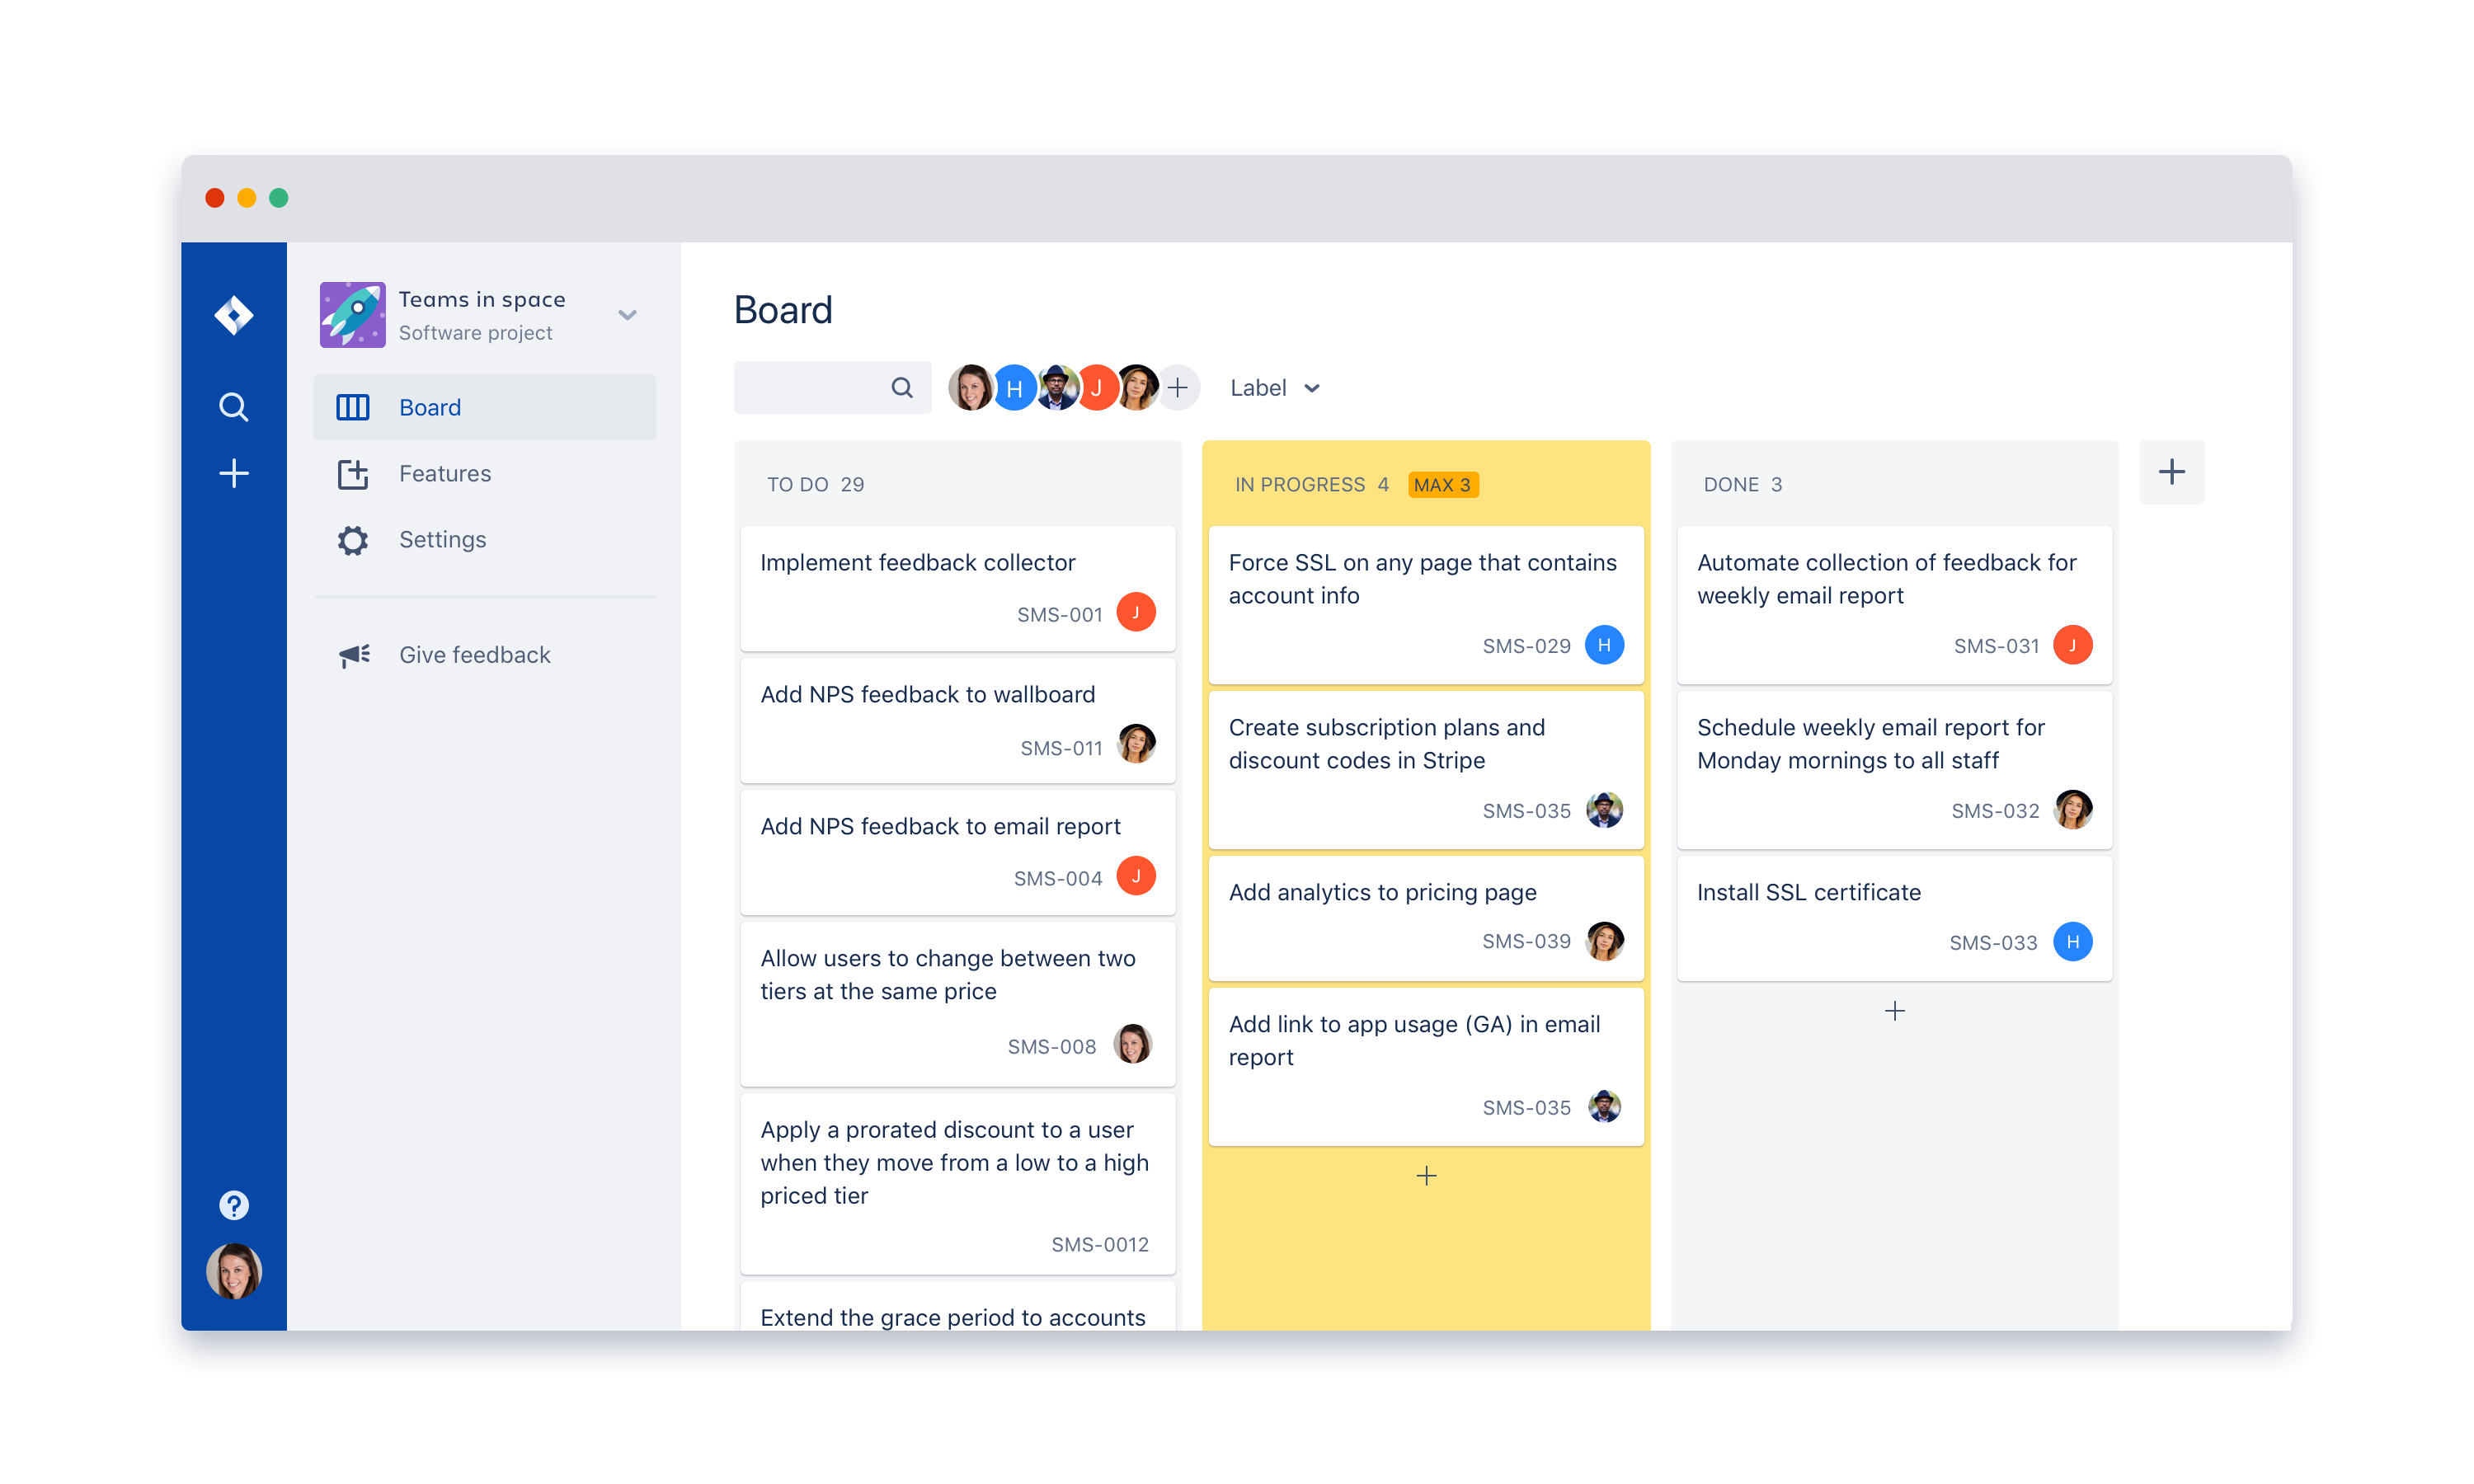
\includegraphics[width=0.95\textwidth]{jira-kanban.png}
    \caption{Kanban Board in Jira}
	\label{fig:kanbanjira}
\end{figure}

Jira ist durch die Grundfunktionalitäten und durch die Möglichkeit der Erweiterung ein sehr mächtiges Werkzeug für Studenten, die noch keine Erfahrungen mit Scrum oder Kanban haben ist es wahrscheinlich schwer den Einstieg zu finden.  Darüber hinaus ist es fraglich ob Studenten den Aufwand bei der Dokumentation innerhalb der Tickets aufwenden werden weil Projekte im universitären Kontext meist sehr kurzlebig sind.  

\begin{figure}[H]
	\centering
	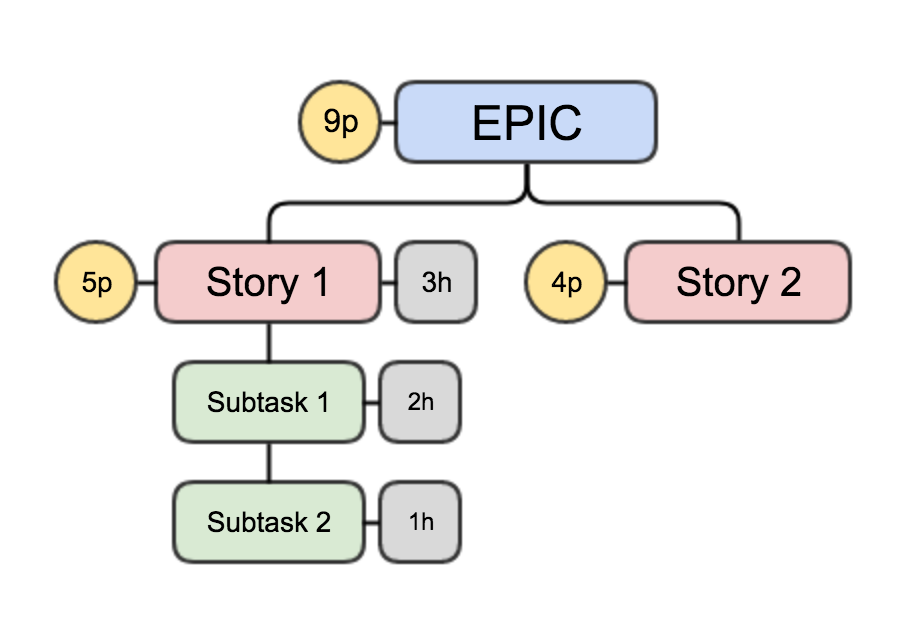
\includegraphics[width=0.95\textwidth]{jira-hierarchie.jpeg}
    \caption{Hierarchie von Tickets in Jira }
	\label{fig:hierarchyjira}
\end{figure}

Ein Dozent wäre aber genau auf die Dokumentation innerhalb der Stories beziehungsweise Tickets angewiesen um nachvollziehen zu können was genau gemacht wird oder wurde. Darüber hinaus müsste der Dozent durch die Strukturen gehen um die dokumentierte Arbeit auf den verschiedenen Ebenen sehen zu können, denn ein Kommentar zum Fortschritt kann in Form eines Kommentars in einem Eric, Story oder Sub-Task stehen. 

\begin{table}[]
    \begin{tabular}{ll}
    Vorteil         & Nachteil                                    \\
    Sehr mächtig    & Hoher Konfigurationsaufwand                 \\
    Durch Plugins erweiterbar   & Setzt Wissen über Kanban oder Scrum vorraus \\
    Workflows innerhalb eines Projekts\\
    können angepasst werden     &                                            
    \end{tabular}
\end{table}

\subsection{Microsoft Project}

Das Erscheinungsjahr von Microsoft Project ist 1984, dieses Produkt ist also schon mehrere Dekaden auf dem Markt.\\
In Microsoft Project wird davon ausgegangen, dass Projekte ein Anfangs und Enddatum haben. Darüber hinaus werden für Tass und Subtasks nicht wie bei Jira Storypunkte vergeben sondern Tage, d.h. eine Aufgabe soll dann zum Beispiel 2 Tage dauern. Microsoft Project bietet drei Ansichten für ein Projekt. \\
Die Ansichten sind
\begin{itemize}
\item Raster  
\item Board  
\item Zeitachse
\end{itemize}
In der Rasteransicht sind alle Aufgaben und deren Unteraufgaben in einer Liste angeordnet. Die Aufgaben und Unteraufgaben können erstellt, sortiert und zugewiesen werden.  

\begin{figure}[H]
	\centering
	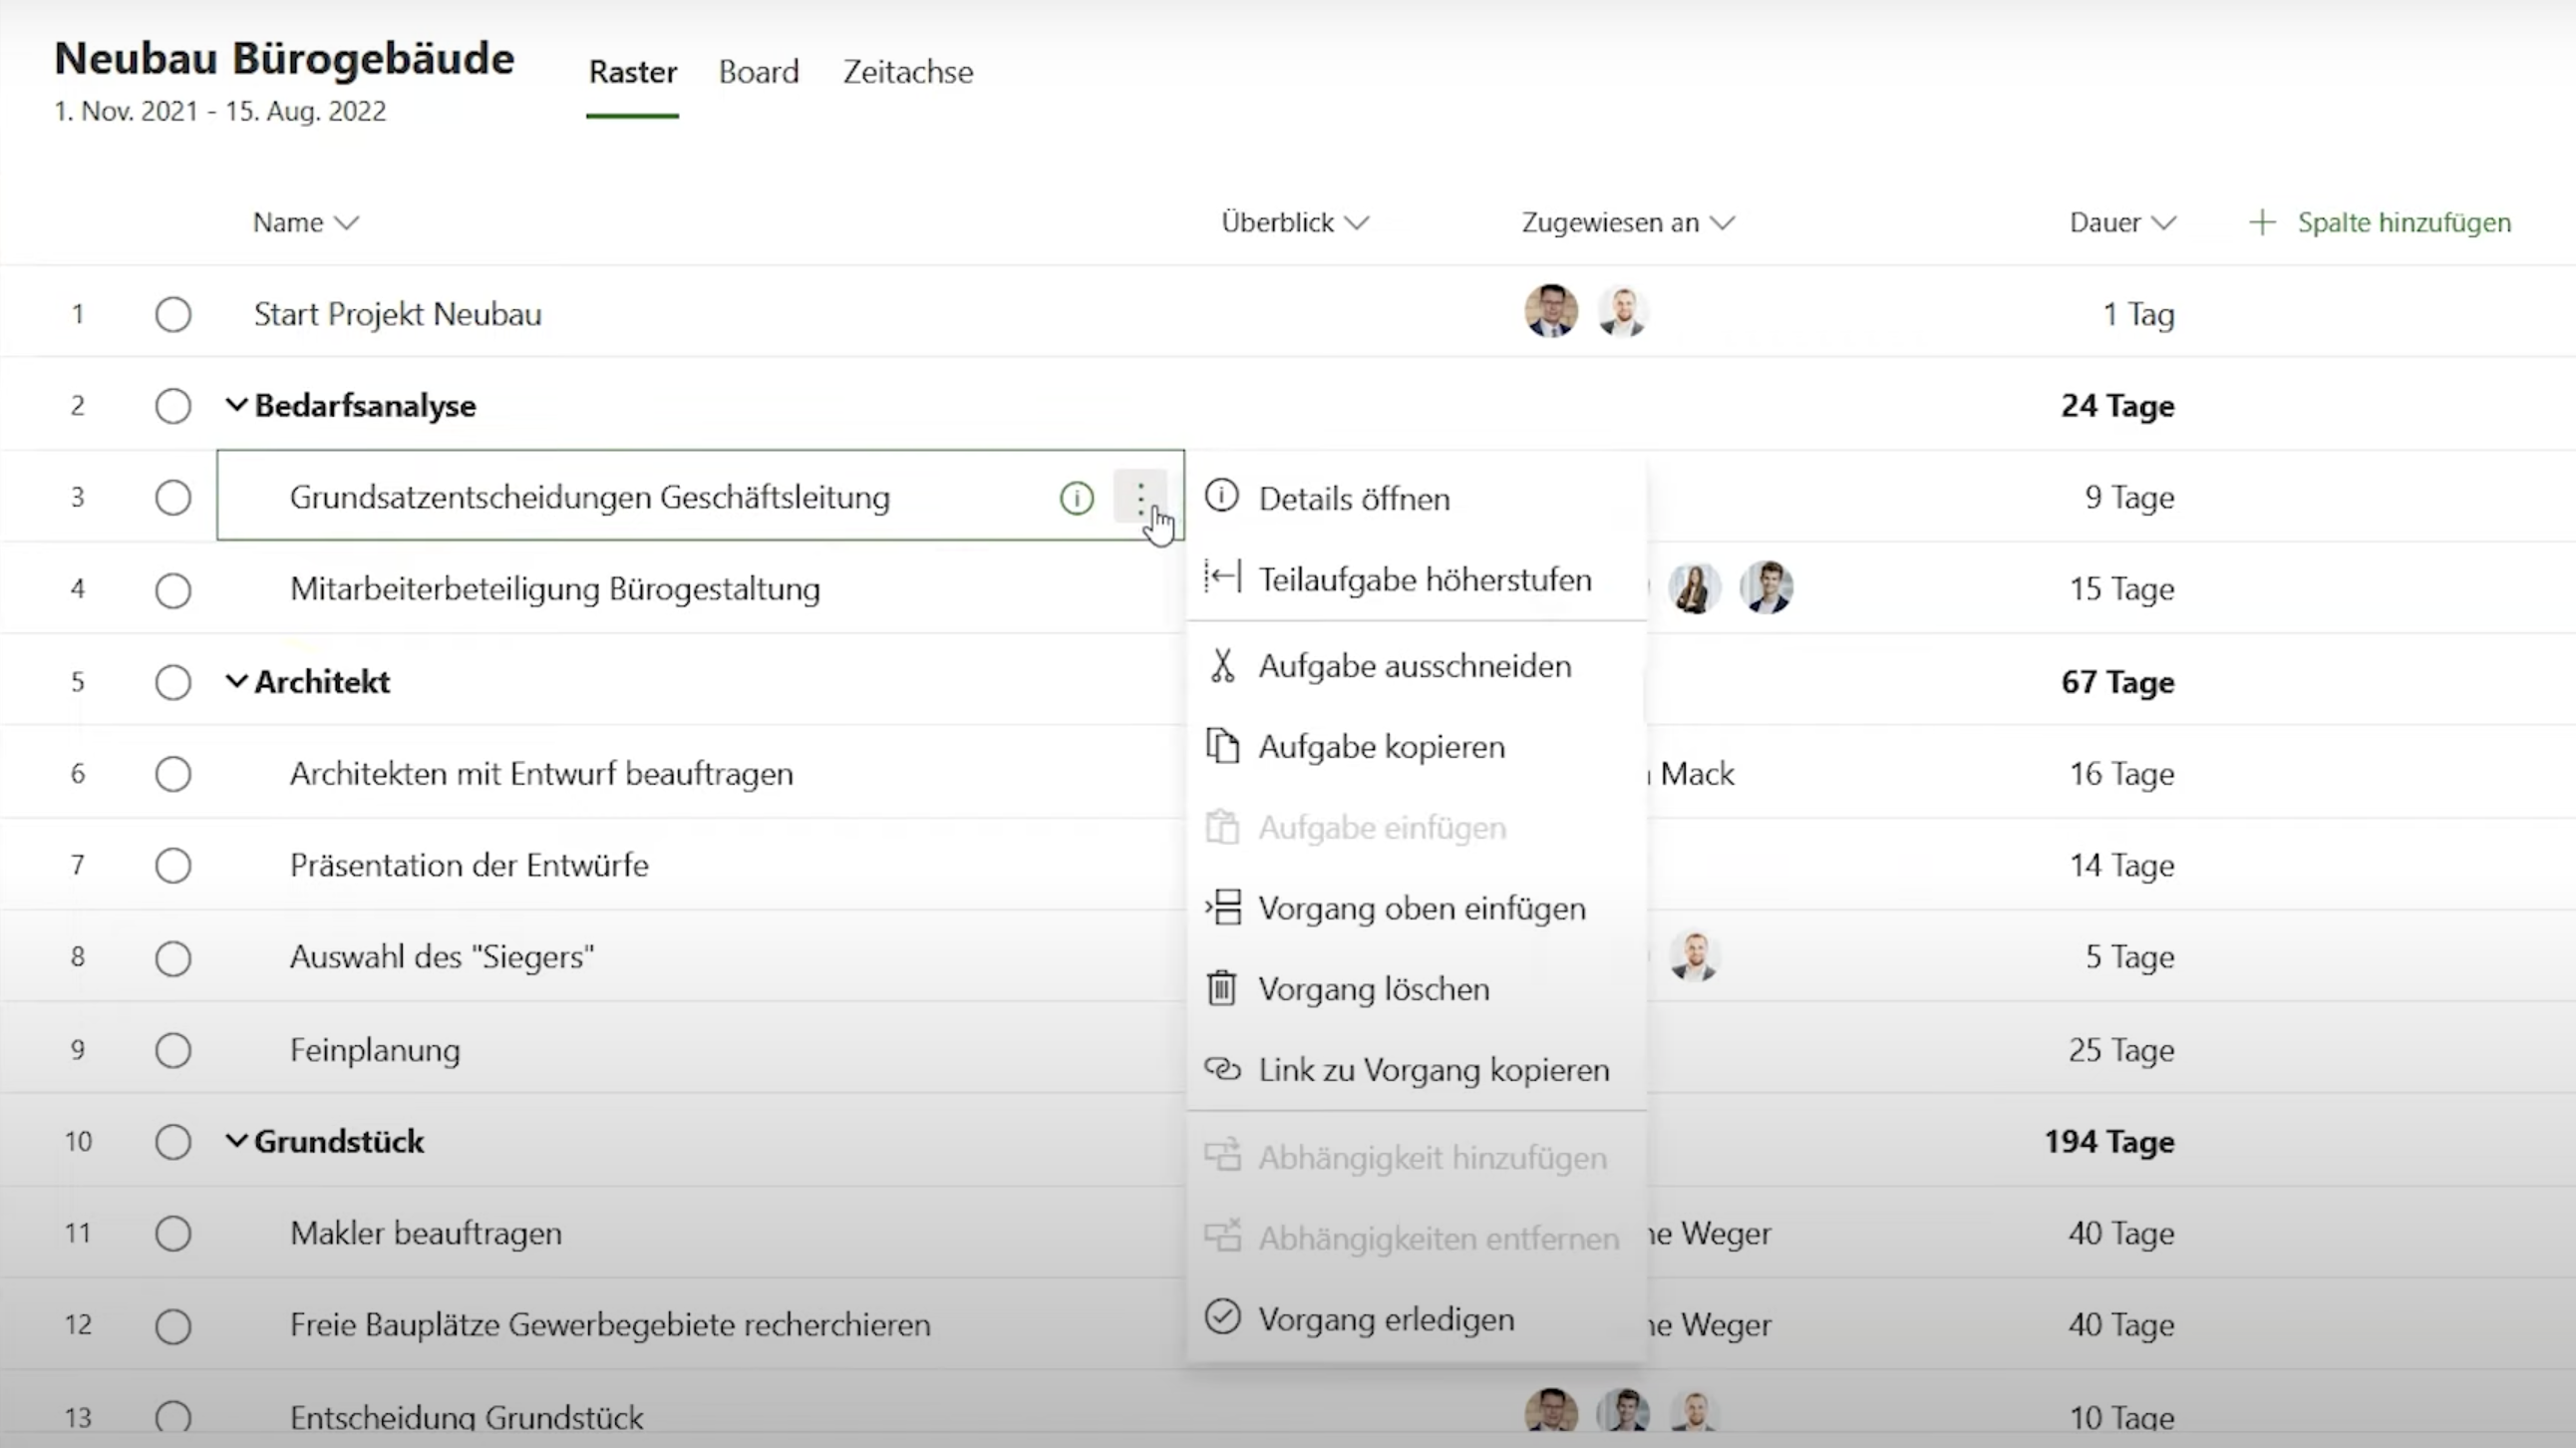
\includegraphics[width=0.95\textwidth]{ms-project-raster.png}
    \caption{Rasteransicht eines Projektes in Microsoft Project}
	\label{fig:rastermsproject}
\end{figure}

Die Aufgaben in Microsoft Project haben als default nur ein Feld für Notizen, d.h. eine Story würde hier nur aus der Headline und einer Notiz bestehen. Der Fokus scheint nicht wie bei Jira auf Softwareprojekte gerichtet zu sein.  

\begin{figure}[H]
	\centering
	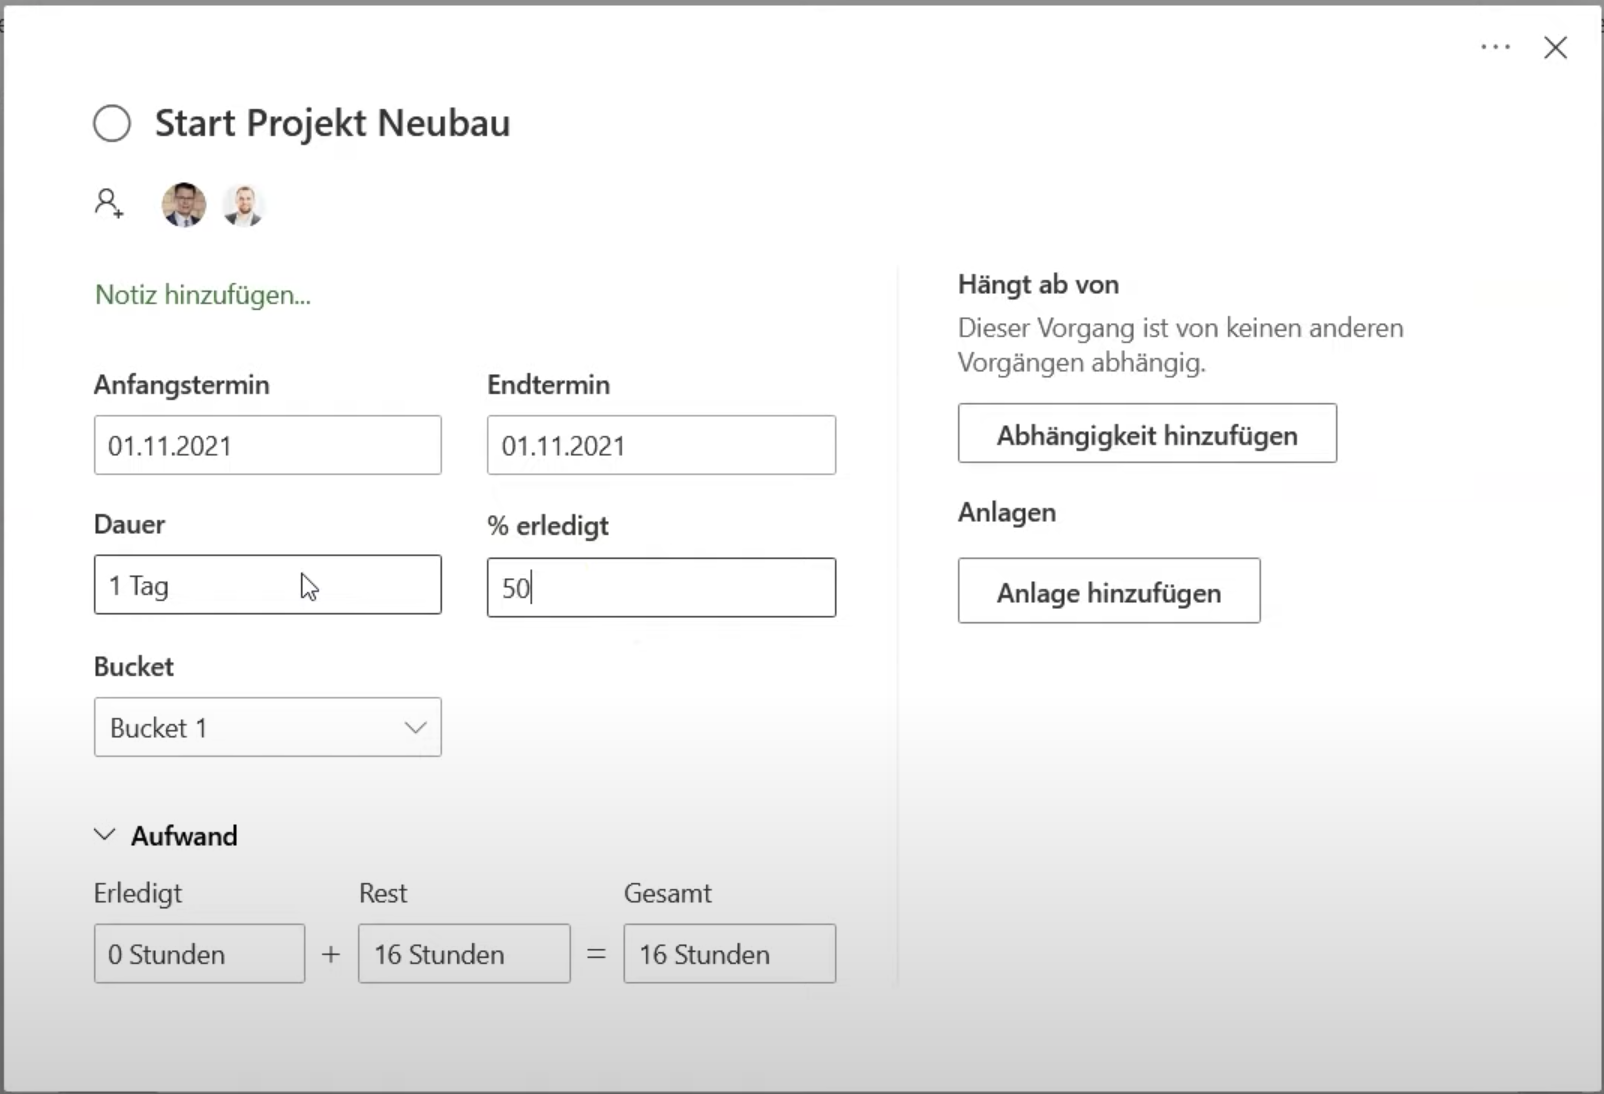
\includegraphics[width=0.95\textwidth]{ms-project-task.png}
    \caption{Eine Aufgabe in Microsoft Project}
	\label{fig:taskmsproject}
\end{figure}

In der Board Ansicht gibt es drei Spalten für die Aufgaben des Projekts\\
\begin{itemize}
    \item Nicht begonnen 
    \item In Arbeit  
    \item Erledigt
\end{itemize}
In dieser Ansicht sind die Aufgaben als Karten dargestellt. Jede Karte hat das Thema, den Bucket, das Fälligkeitsdatum, den Prozentualen Fortschritt und die Icons mit Bildern der Personen, die diese Aufgabe zugewiesen haben. Das Kanban Board kann aber konfiguriert werden um zum Beispiel mehr Spalten oder andere Informationen in den Karten anzuzeigen.\\

\begin{figure}[H]
	\centering
	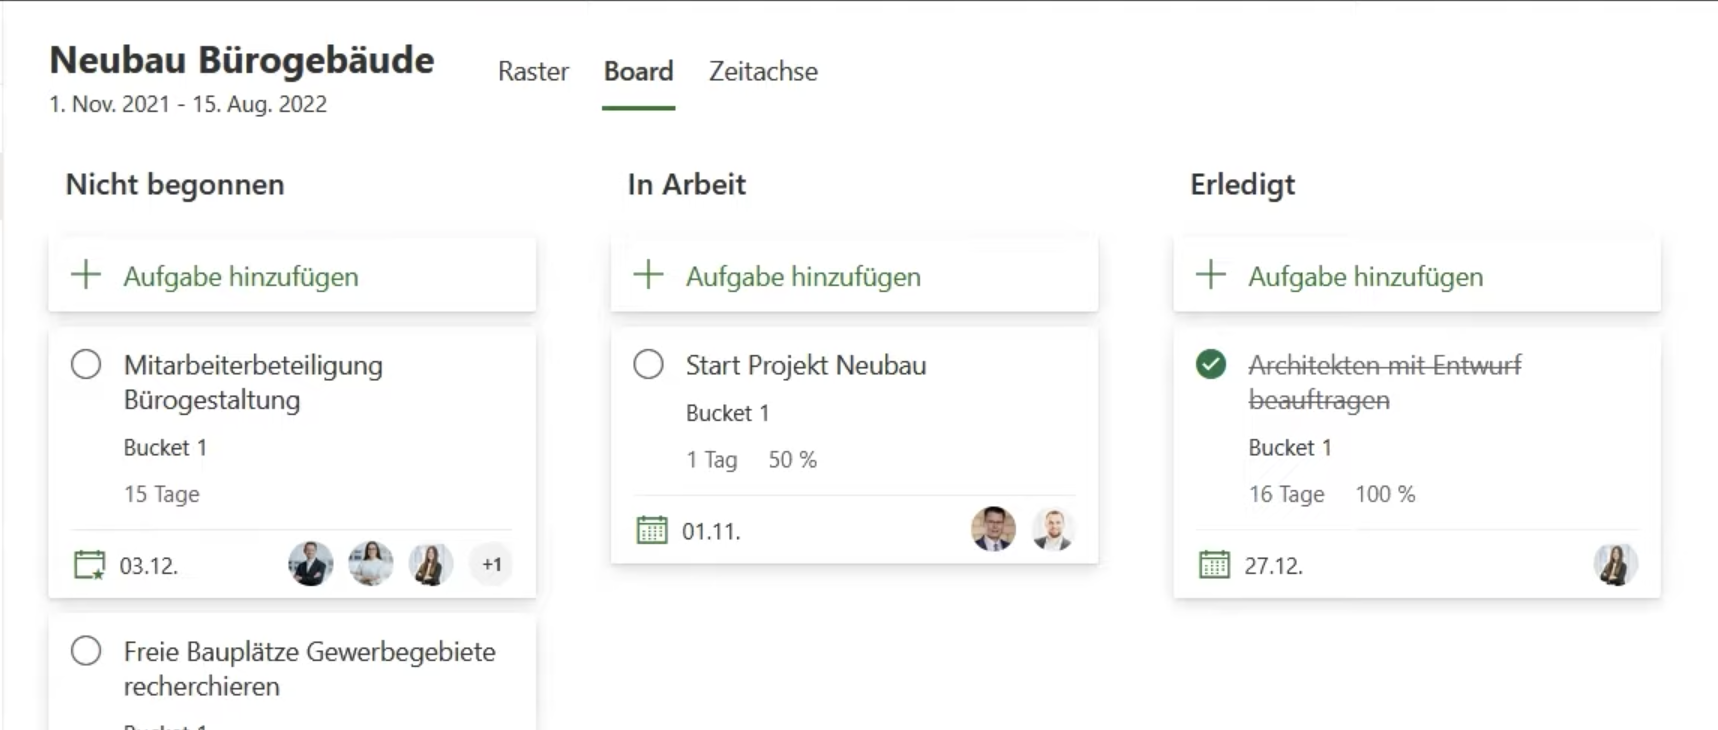
\includegraphics[width=0.95\textwidth]{ms-project-kanban.png}
    \caption{Kanban Board in Microsoft Project}
	\label{fig:kanbanmsproject}
\end{figure}

In der Zeitachsen Ansicht wird auf der linken Seite die Liste mit den Aufgaben angezeigt und auf der rechten Seite wird ein Graph aus den Aufgaben erstellt. Dabei hat jede Aufgabe eine Zeile und eine Länge auf der Zeitachse.\\
Abhängigkeiten werden durch Pfeile dargestellt. Ein Pfeil geht von links nach rechts, d.h. die Abhängigkeiten werden im zeitlichen Ablauf dargestellt. Die Aufgaben können in dieser Ansicht auf der Zeitachse verlängert oder verkürzt werden.\\

\begin{figure}[H]
	\centering
	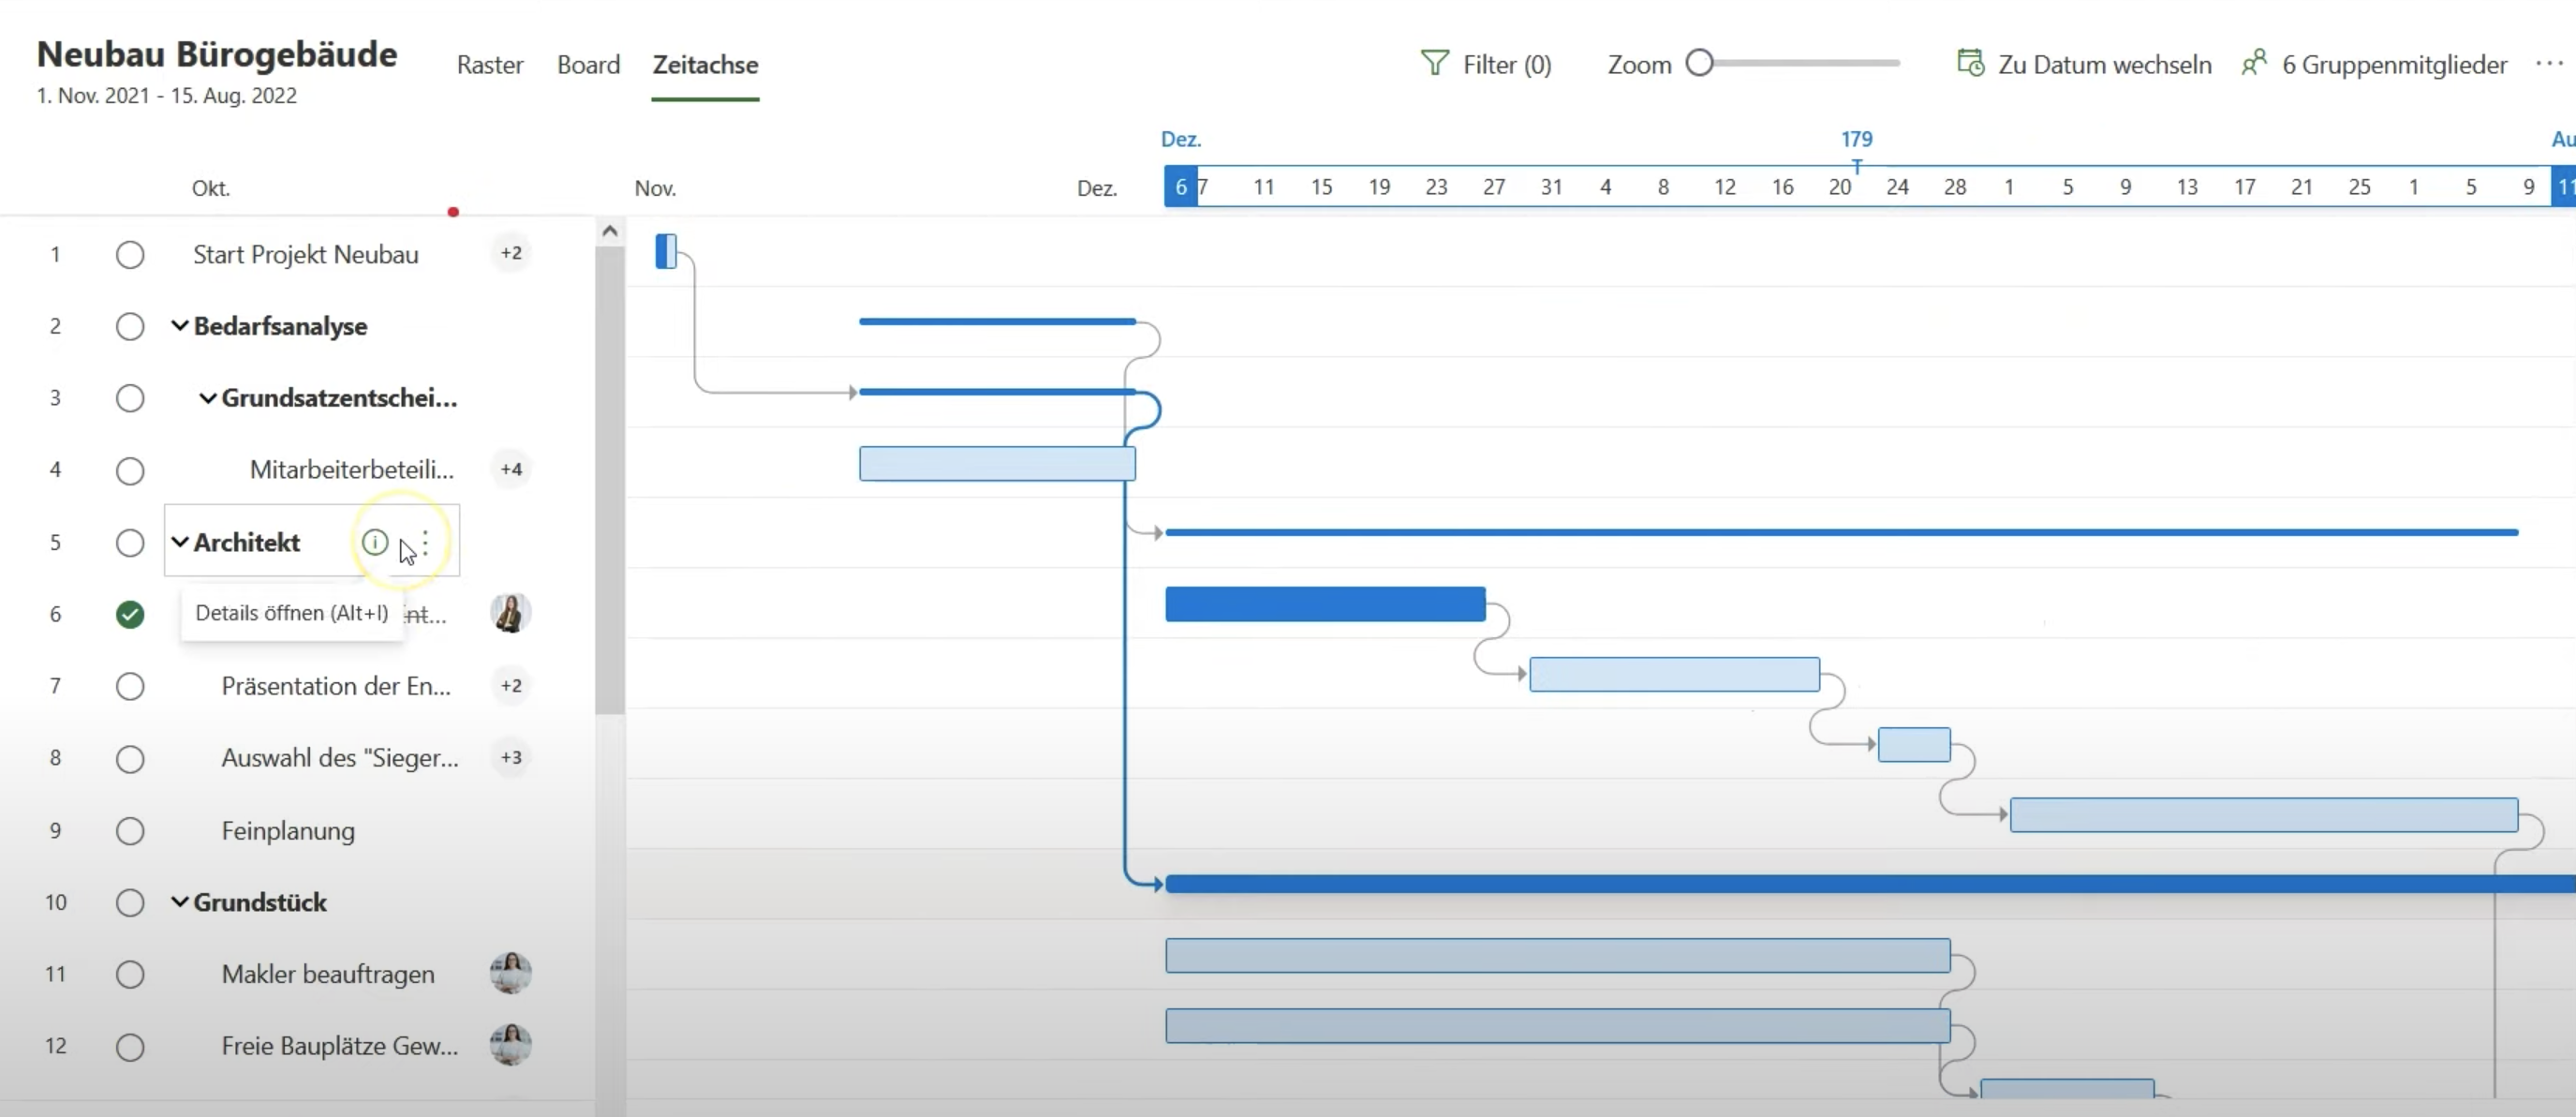
\includegraphics[width=0.95\textwidth]{ms-project-timeline.png}
    \caption{Zeitachse in Microsoft Project}
	\label{fig:timelinemsproject}
\end{figure}

Für Projektleiter oder Abteilungsleiter gibt es auch eine Ansicht für Roadmaps in denen man auf einer Zeitachse mehrere Projekte zu sehen. Es können auch Aufgaben auf dieser Ebene hinzugefügt werden. Diese Ansicht wäre für Dozenten interessant. Zusammenfassend lässt sich sagen, dass Microsoft von den Features interessant für Studentenprojekte ist allerdings braucht jeder Student dann eine Lizenz für diese Software, da normale Office 365 Nutzer nur Lesezugriff haben. Für Softwareprojekte stellt sich auch noch die Frage des Konfigurationsaufwands um zum Beispiel eine Story korrekt darzustellen in der dann mehr als eine Notiz drin ist wie zum Beispiel Designs oder Testfälle.  Eine Funktion für ein Daily oder Weekly Meeting gibt es als Default nicht, d.h. es müsste alles manuell in den einzelnen Aufgaben dokumentiert werden, was auf der Seite der Dozenten einen erheblichen Mehraufwand darstellt.  

\subsection{Asana Kanban}

Asana wurde 2008 gegründet und ist seit 2012 kommerziell davor war es ostenlos. In Asana gibt es wie bei Microsoft Project verschiedenen Ansichten. Beim Erstellen des Projekts wird eine Default Ansicht ausgewählt dabei kann man aus 4 verschiednen Optionen wählen:
\begin{itemize}
    \item List 
    \item Board 
    \item Timeline  
    \item Calendar 
\end{itemize}

Im Kanban Board sieht man wie bei Jira oder Microsoft Project als Default 3 Spalten:
\begin{itemize}
    \item To Do
    \item In Progress
    \item Complete
\end{itemize}

Innerhalb der Tasks kann man sehen welcher Person das Task zugewiesen wurde, welche Zeitraum vorgesehen ist.

\begin{figure}[H]
	\centering
	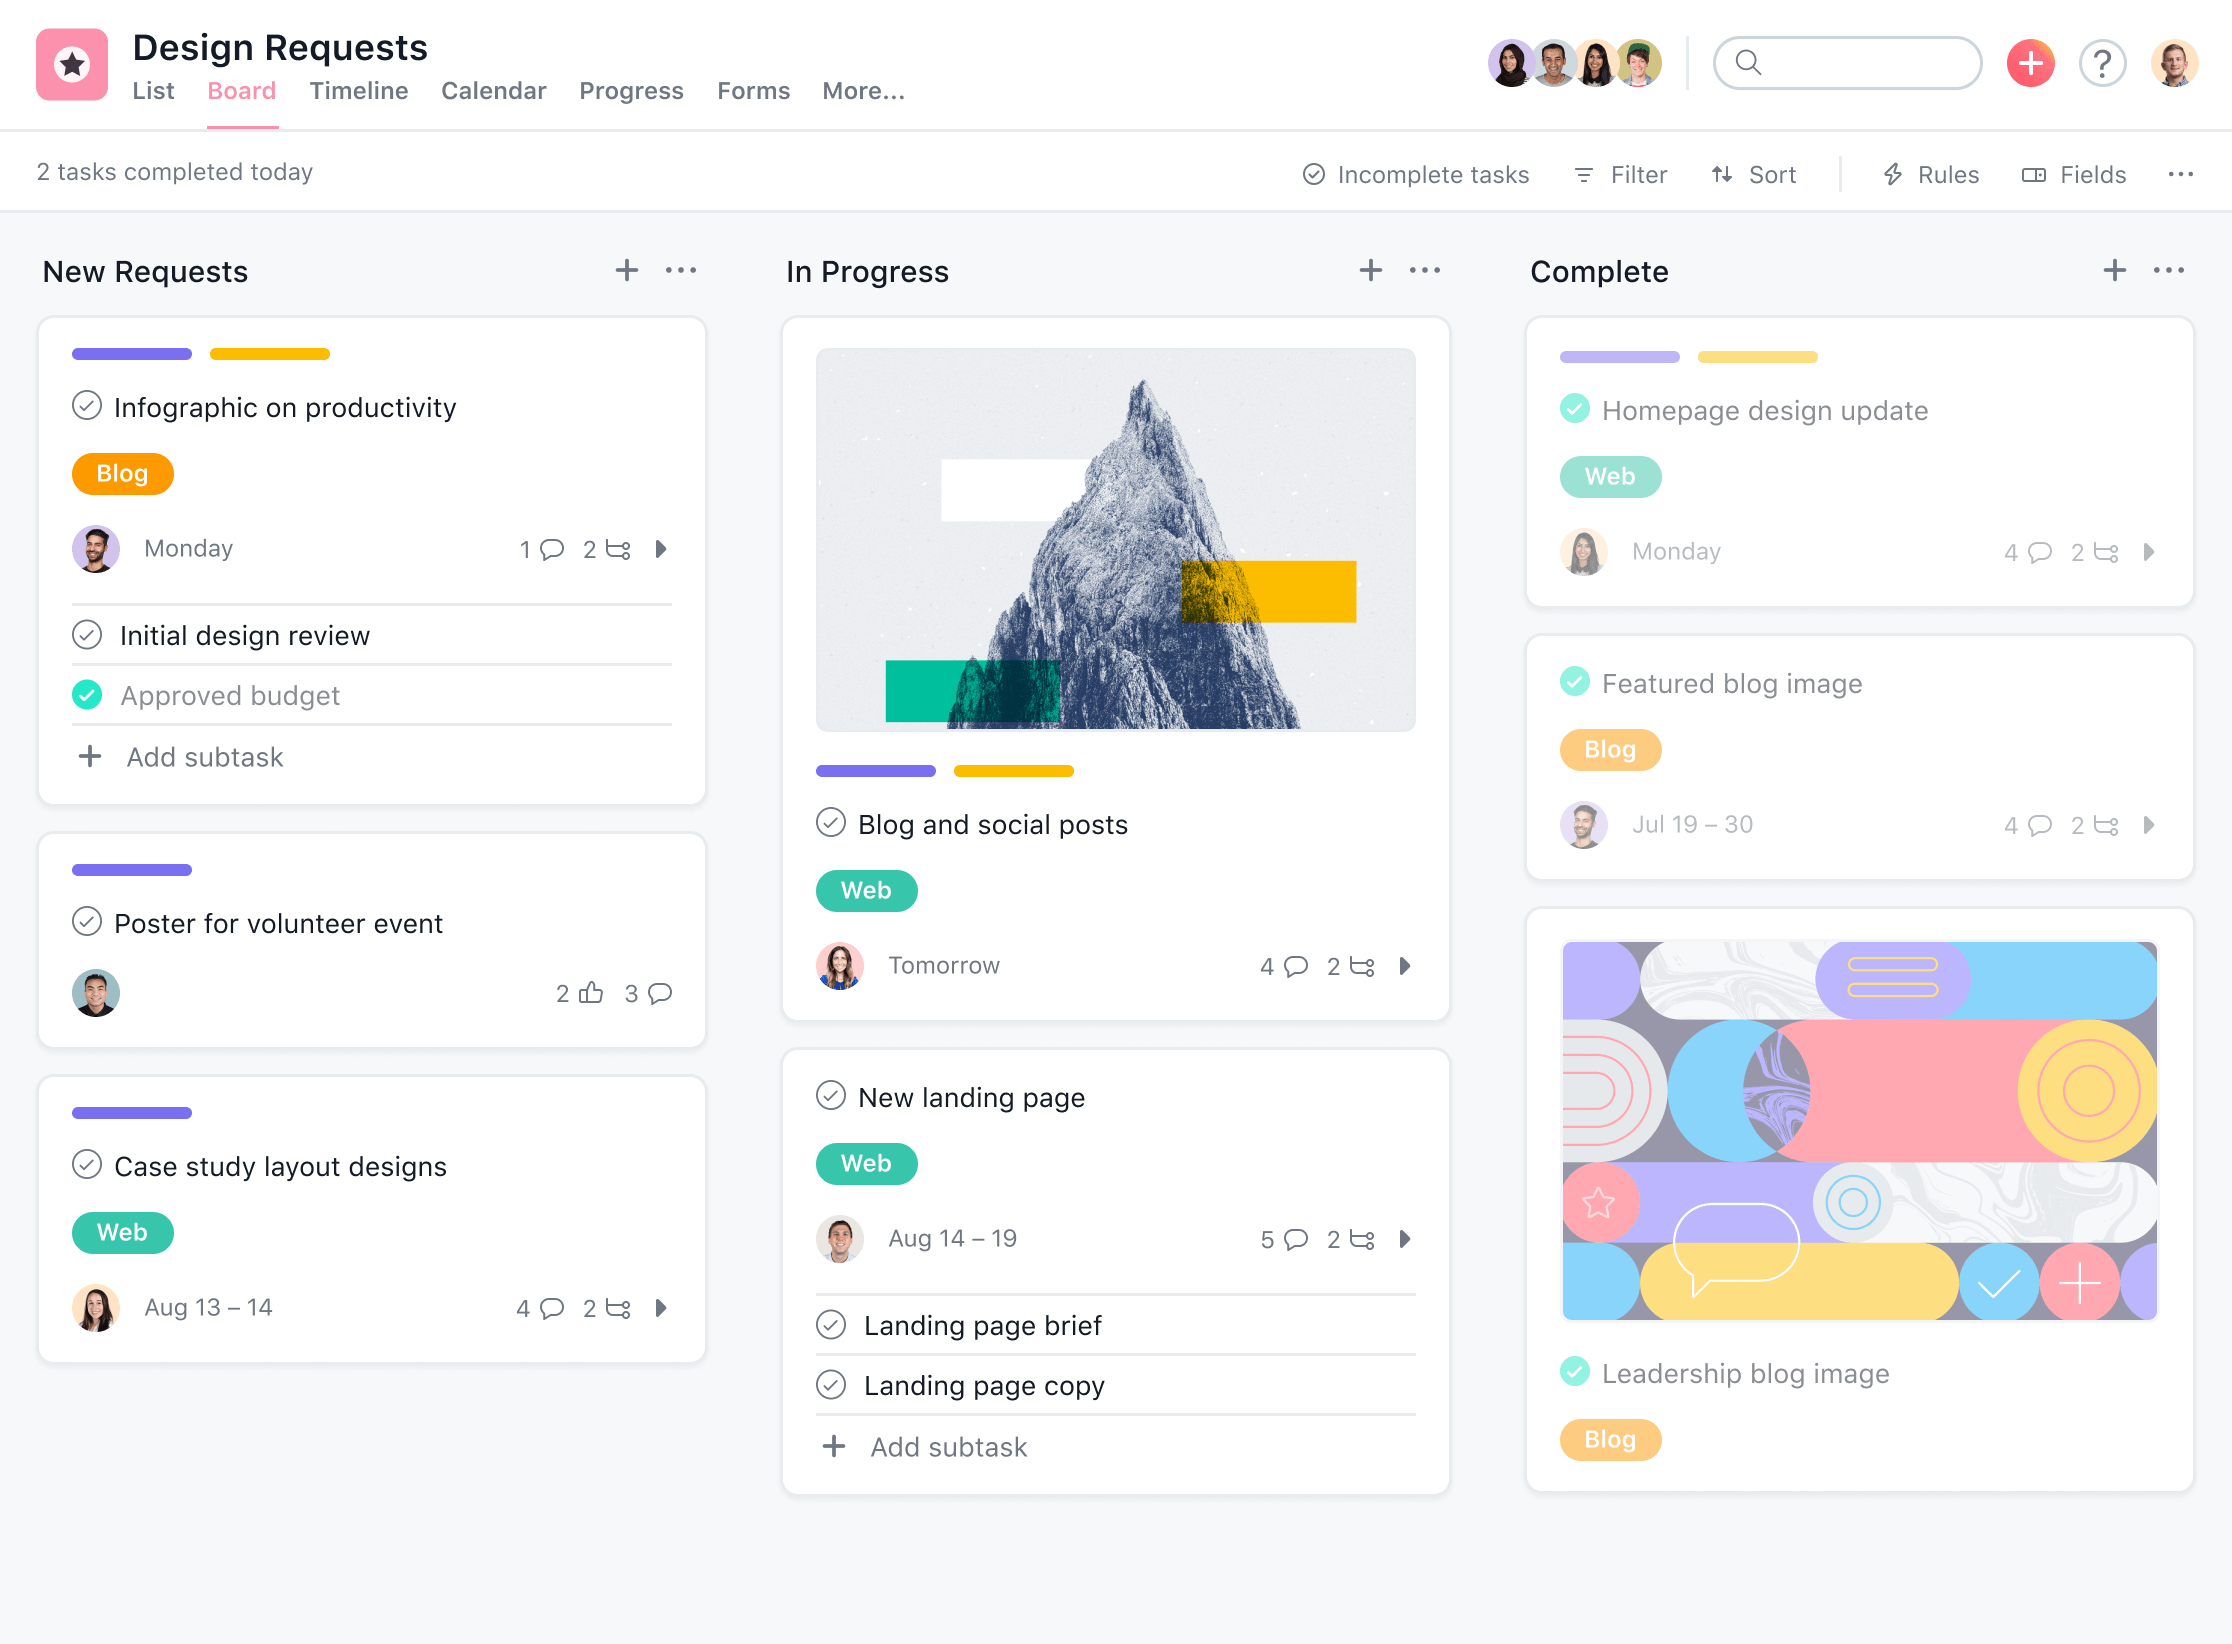
\includegraphics[width=0.95\textwidth]{asana-kanban.png}
    \caption{Kanban Board in Asana}
	\label{fig:kanbanasana}
\end{figure}


Außerdem sieht man die Subtasks und falls Bilder hinzugefügt wurden eine Vorschau des Bildes in dem Ticket. Für Meetings gibt es in Asana „Meeting Agenda Projects“. Es gibt hier zwei mögliche Ansichten List und Board. In der List Ansicht wird für jedes Punkt der Agenda ein Task hinzugefügt. Es können dann als nächstes die Teilnehmer zu dem Meeting Projekt hinzugefügt werden. Neue Tasks können dann während des Meetings hinzugefügt werden.

\begin{figure}[H]
	\centering
	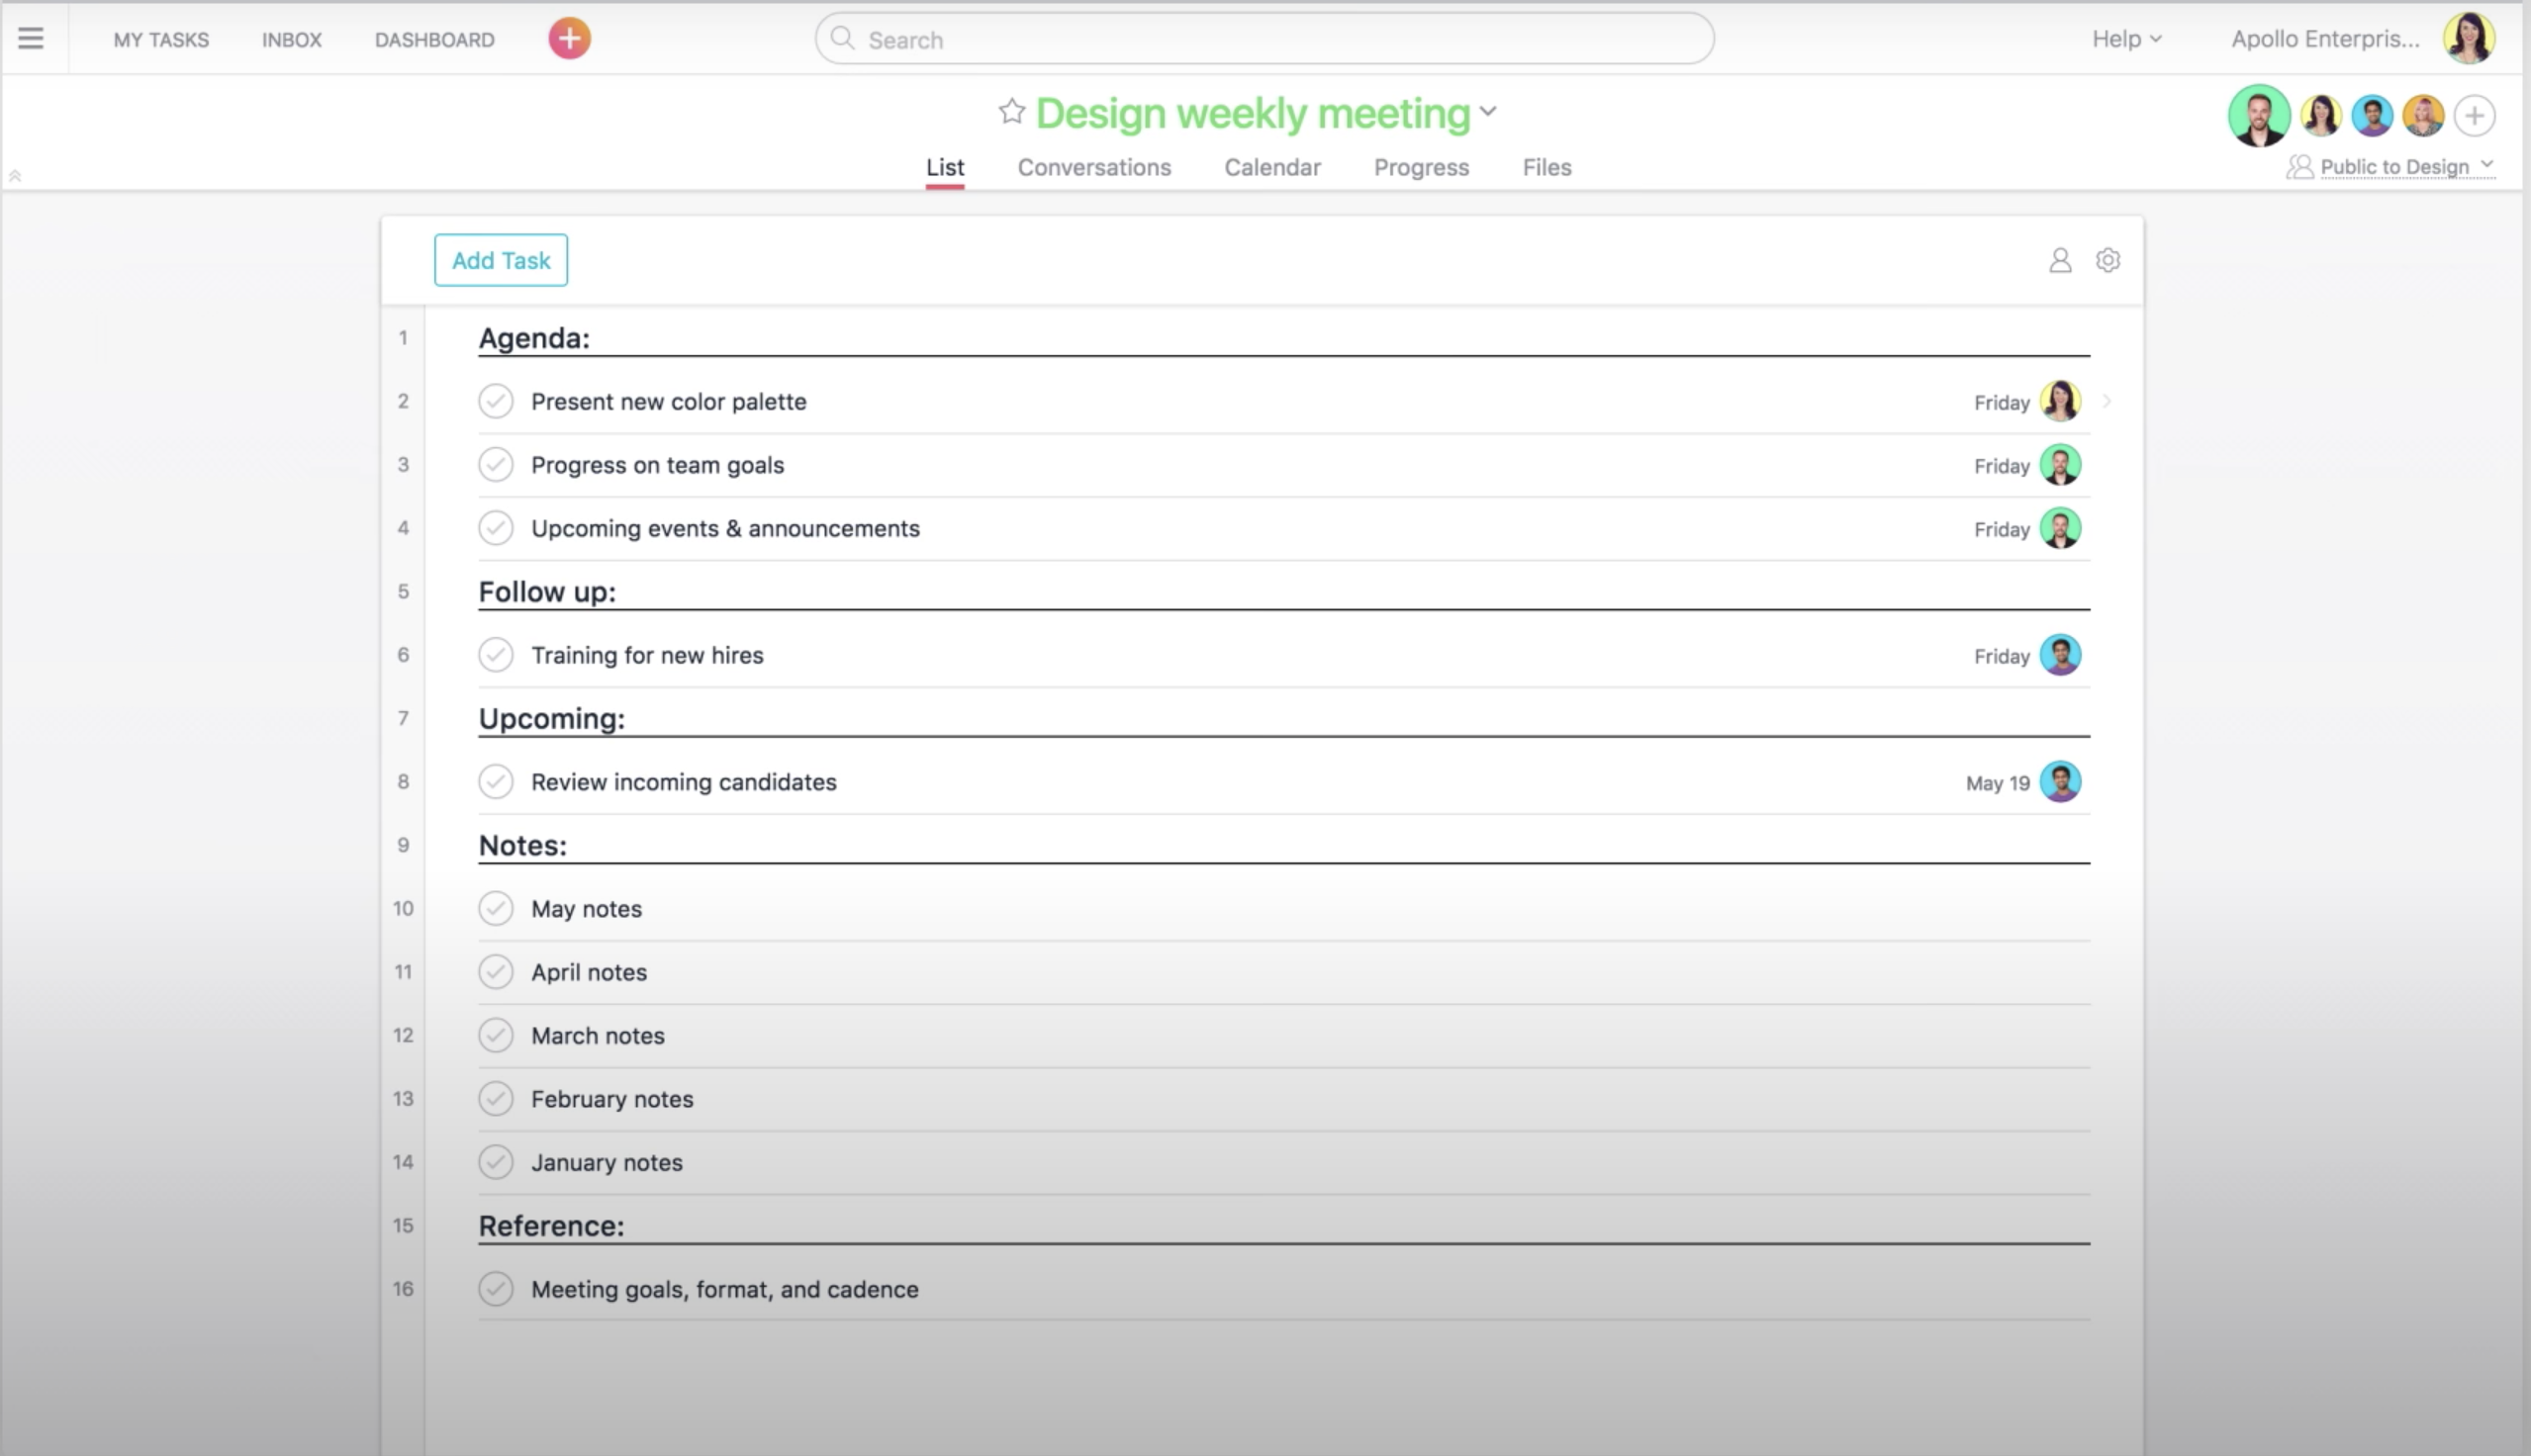
\includegraphics[width=0.95\textwidth]{asana-weekly.png}
    \caption{Weekly in Asana}
	\label{fig:weeklyasana}
\end{figure}

Die Tasks in dem Meeting Projekt können per Drag \& Drop in der Agenda bewegt werden. Fertige Tasks können abgehakt werden. Für die Tasks kann jeweils ein Fälligkeitsdatum gesetzt werden.\\
Asana ist von den vorgestellten Lösungen am interessantesten allerdings bietet es nicht die Möglichkeit automatisch ein wiederkehrendes Meeting zu konfigurieren so wie es Studenten und Dozenten in einem universitären Projekt brauchen zumindest nicht out of the box.

\section{Ergebnis}

Welche Stärken und Schwächen haben die Konkurrenzprodukte?\\

Zunächst lässt sich feststellen, dass keines der analysierten Konkurrenzprodukte ein ähnliches Feature hat. Der Grund dafür wird in dem Fokus auf Unternehmen liegen. Es gibt Features für Reports aber auch hier haben sie ein anderes Ziel als wir es im universitären Kontext brauchen, denn in einem Unternehmen werden Mitarbeiter zwar bewertet aber nicht in der gleichen Weise wie in einer Lehranstalt.\\
Jira richtet sich an agil arbeitenden Firmen mit einem Fokus auf Scrum und Kanban. Die Projekte haben hier normalerweise keine feste Deadline. Die Schätzungen durch das Team sind essentiell in Jira, denn ohne sie funktionieren eine Reihe von Reports nicht. Ob Studenten ohne Vorwissen in der Lage sind Schätzungen abzugeben ist fraglich und es würde sich dann auch die Frage 
nach Plannings und einem Scrum Master stellen.\\
Microsoft Project richtet sich an Unternehmen mit Projekten, die nach dem Wasserfall Prinzip abgearbeitet werden, deswegen haben Tasks dort auch per default ein Fälligkeitsdatum. Im universitären Kontext trifft das schon eher auf Projekte zu, wenn sie zum Beispiel innerhalb eines laufenden Semesters bearbeitet werden müssen.  Allerdings hat man hier das Problem mit den Lizenzen, da jedes Teammitglied eine aktive Lizenz braucht um mehr zu tun als zu lesen. Falls es von der jeweiligen Universität eine Partnerschaft gibt könnte es funktionieren Microsoft Projects einzusetzen allerdings bietet es kein Feature um Weekly Meetings so zu dokumentieren, dass es schnell und einfach durch den Dozenten erfasst werden kann.\\
Asana ist eine Mischung aus Jira und Microsoft Project, denn man hat hier auch die verschieden Ansichten aber einen stärkeren Fokus auf agiles Arbeiten als bei Microsoft Project. Im Gegensatz zu den andren beiden gibt es hier die Möglichkeit ein extra Meeting Project aufzusetzen allerdings bietet diese Projektart auch nicht was wir brauchen beziehungsweise entwickeln wollen. 

\clearpage